\section{Impact on SK oscillation analyses}
\red{finish me}
\begin{table}
	\begin{tabular}{l | c}
		\hline
		\hline
		Parameter & Value \\
		\hline
		$\sin2\theta_{12}$ & 0.304 \\
		$\sin2\theta_{23}$ & 0.528 \\
		$\sin2\theta_{13}$ & 0.0219 \\
		$\Delta m^2_{12}$  & $7.53\times10^{-5} \text{ eV}^2$ \\
		$\Delta m^2_{23}$  & $2.509\times10^{-3} \text{ eV}^2$ \\
		$\delta_{cp}$ & -1.601 \\
		\hline
		\hline
	\end{tabular}
\caption{Oscillation parameters used to produce nominal event rates at SK}
\label{tab:osc_pars}
\end{table}

% from /tmp/ts-out.2tydjK on heppc105, June 1, 10,000 throws
\begin{table}
	\begin{tabular}{l | c c | c c}
		\hline
		\hline
		Sample & \multicolumn{2}{c|}{Event rate} & \multicolumn{2}{c}{$\delta N/N$ (\%)} \\
		& Pre-fit & Post-fit & Pre-fit & Post-fit \\
		\hline
		$1\text{R}\mu$ & $249.86\pm34.96$ & $262.59\pm8.03$ & 13.99 & 3.06 \\
		$1\text{R}e$ & $65.62\pm9.95$ & $72.13\pm2.88$ & 15.16 &  3.99   \\
		$1\text{R}e \text{ 1d}e$ & $7.70\pm0.93$ & $6.73\pm0.32$ & 12.08 & 4.75  \\
		
		$1\text{R}\mu \text{ RHC}$ & $61.50\pm7.21$ & $62.57\pm1.73$ & 11.72 & 2.76 \\
		$1\text{R}e \text{ RHC}$ & $7.64\pm0.95$ & $7.72\pm0.32$ & 12.43 & 4.15  \\
		\hline
		\hline
	\end{tabular}
\caption{T2K-SK event rates and uncertainties from flux and interaction systematics with and without near-detector constraints from this analysis (not including SK and oscillation parameter errors)}
\label{tab:sk_evt_rates_2017}
\end{table}


\begin{figure}[h]
	\begin{subfigure}[t]{0.32\textwidth}
		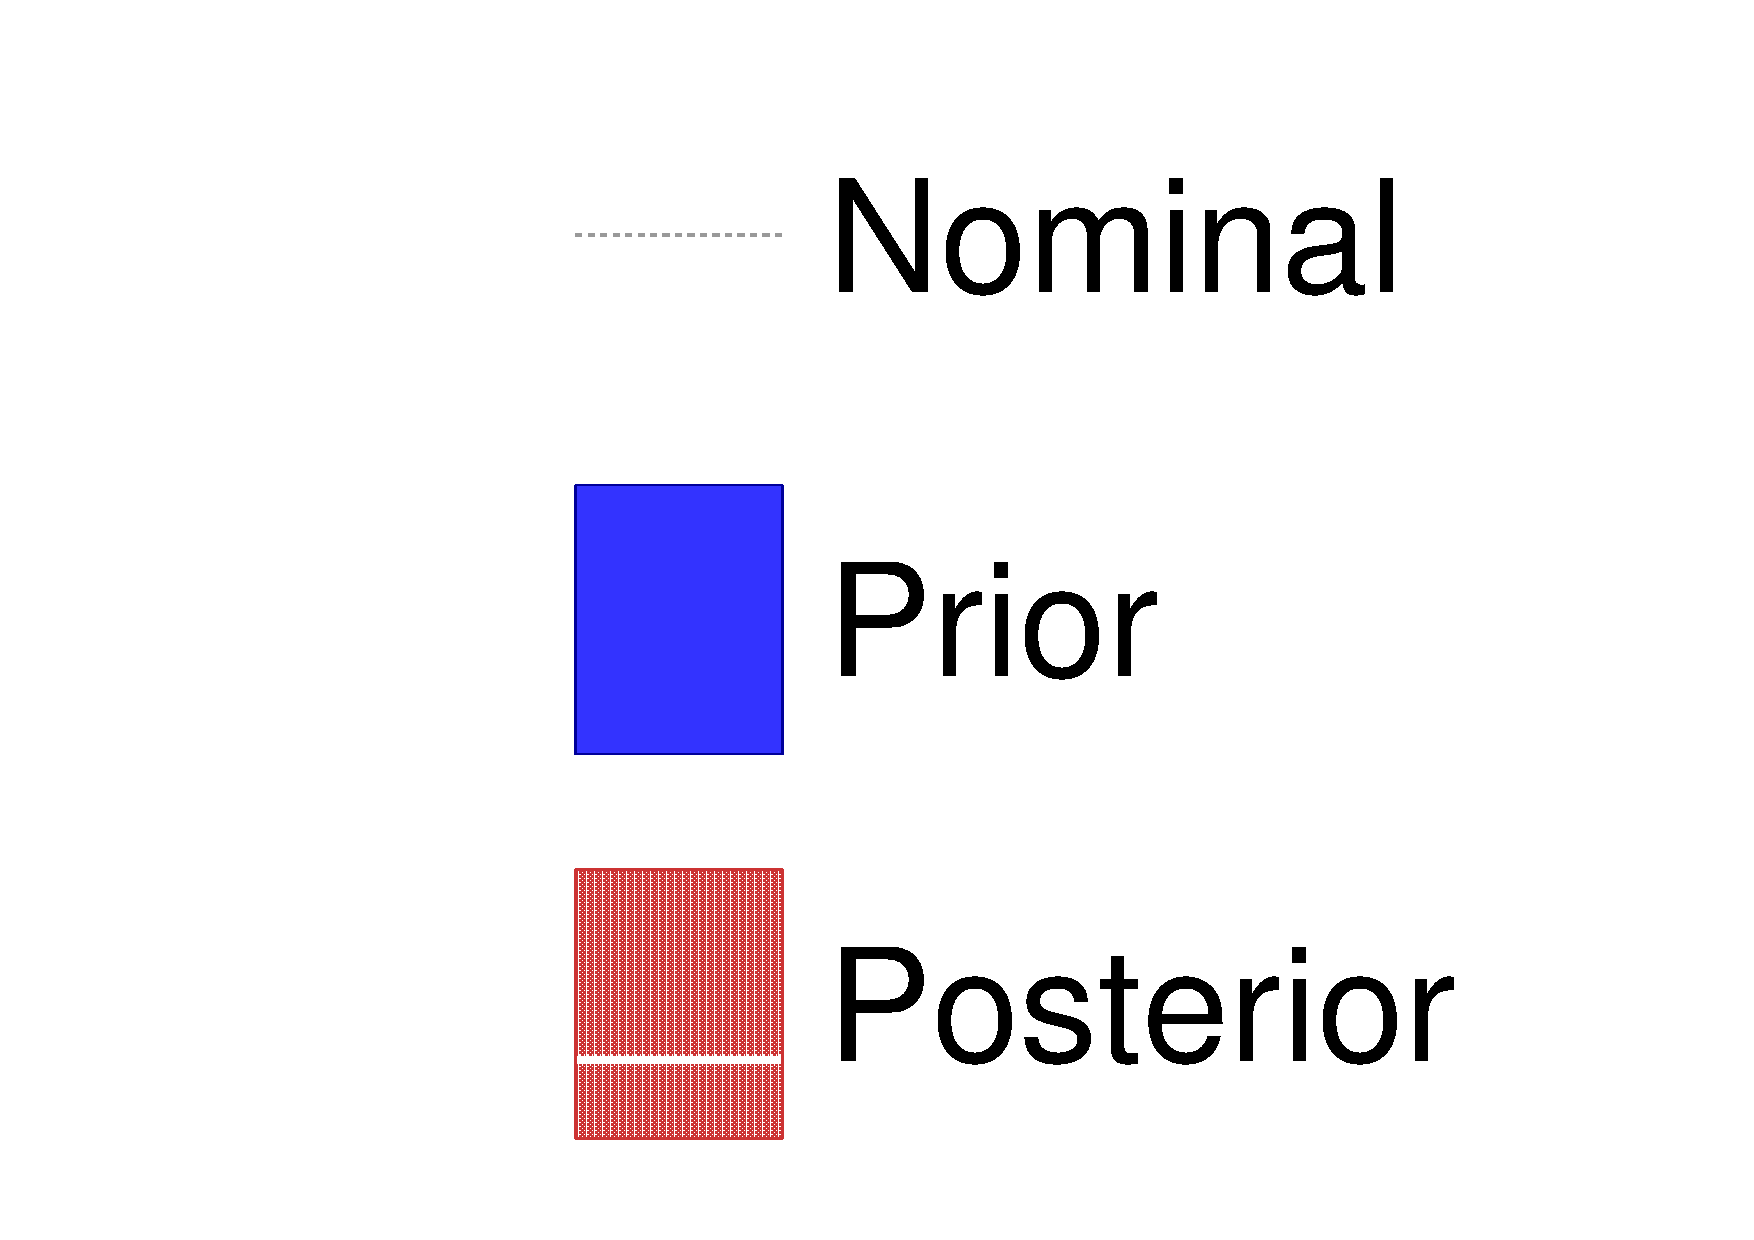
\includegraphics[width=\textwidth, trim={0mm 0mm 0mm 0mm}, clip, page=1]{figures/mach3/data/prior_error_1june_try_2017_fit_on_sk_spectra}
	\end{subfigure}
	\begin{subfigure}[t]{0.32\textwidth}
		\includegraphics[width=\textwidth, trim={0mm 0mm 0mm 0mm}, clip, page=5]{figures/mach3/data/prior_error_1june_try_2017_fit_on_sk_spectra}
	\end{subfigure}
	\begin{subfigure}[t]{0.32\textwidth}
		\includegraphics[width=\textwidth, trim={0mm 0mm 0mm 0mm}, clip, page=6]{figures/mach3/data/prior_error_1june_try_2017_fit_on_sk_spectra}
	\end{subfigure}
	
	\begin{subfigure}[t]{0.32\textwidth}
		\includegraphics[width=\textwidth, trim={0mm 0mm 0mm 0mm}, clip, page=2]{figures/mach3/data/prior_error_1june_try_2017_fit_on_sk_spectra}
	\end{subfigure}
	\begin{subfigure}[t]{0.32\textwidth}
		\includegraphics[width=\textwidth, trim={0mm 0mm 0mm 0mm}, clip, page=3]{figures/mach3/data/prior_error_1june_try_2017_fit_on_sk_spectra}
	\end{subfigure}
	\begin{subfigure}[t]{0.32\textwidth}
		\includegraphics[width=\textwidth, trim={0mm 0mm 0mm 0mm}, clip, page=4]{figures/mach3/data/prior_error_1june_try_2017_fit_on_sk_spectra}
	\end{subfigure}
	
	\caption{Impact of the full fit on SK spectra compared to the prior}
	\label{fig:sk_2017}
\end{figure}


\subsection{Alternative studies impact}
Here we investigate the impact of the alternative studies that had the largest effect on the ND280 fit and propagate the results to SK. For the oscillation parameters we fix them to those in \autoref{tab:osc_pars} and the SK detector parameters are set to their prior central values and are not varied.

The procedure mimics that of the posterior predictive method, in which MCMC steps are randomly selected after burn-in to give a parameter set $\vec{x}$, used to reweight the Monte-Carlo prediction which is filled in a two-dimensional histogram ($N_{toys}$ vs $E_{rec}$ here). A Gaussian is then fit to the bin-by-bin distributions and the mean and rms is extracted and taken as the central value and 1$\sigma$.

\subsubsection{2015-like}
The 2015-like parameterisation fixed 2p2h shape and BeRPA to their prior values and did not vary them in the fit. This roughly reproduced the results from the ND280 fit from 2015\cite{t2k_2015}. 

\autoref{fig:sk_2015like} shows the $E_{reco}$ distributions for the five samples at Super-Kamiokande. We note the largest difference in spectrum is in the $1\text{R}\mu$ sample between $0.2 < E_{rec} < 0.5\text{ GeV}$: the region which is sensitive to oscillation parameters (mostly $\theta_{23}$ and $\Delta m^2_{23}$ or $\Delta m^2_{32}$). The shift is less than 1$\sigma$ of the full data fit. The $1\text{R}e$ selection has a consistently lower event rate for the 2015-like fit, which has an impact on $\theta_{13}$ primarily, and the effect on the $1\text{R}e1\text{d}e$ selection is opposite. The RHC selections are entirely consistent and see no deviations from each other.
\begin{figure}[h]
	\begin{subfigure}[t]{0.32\textwidth}
		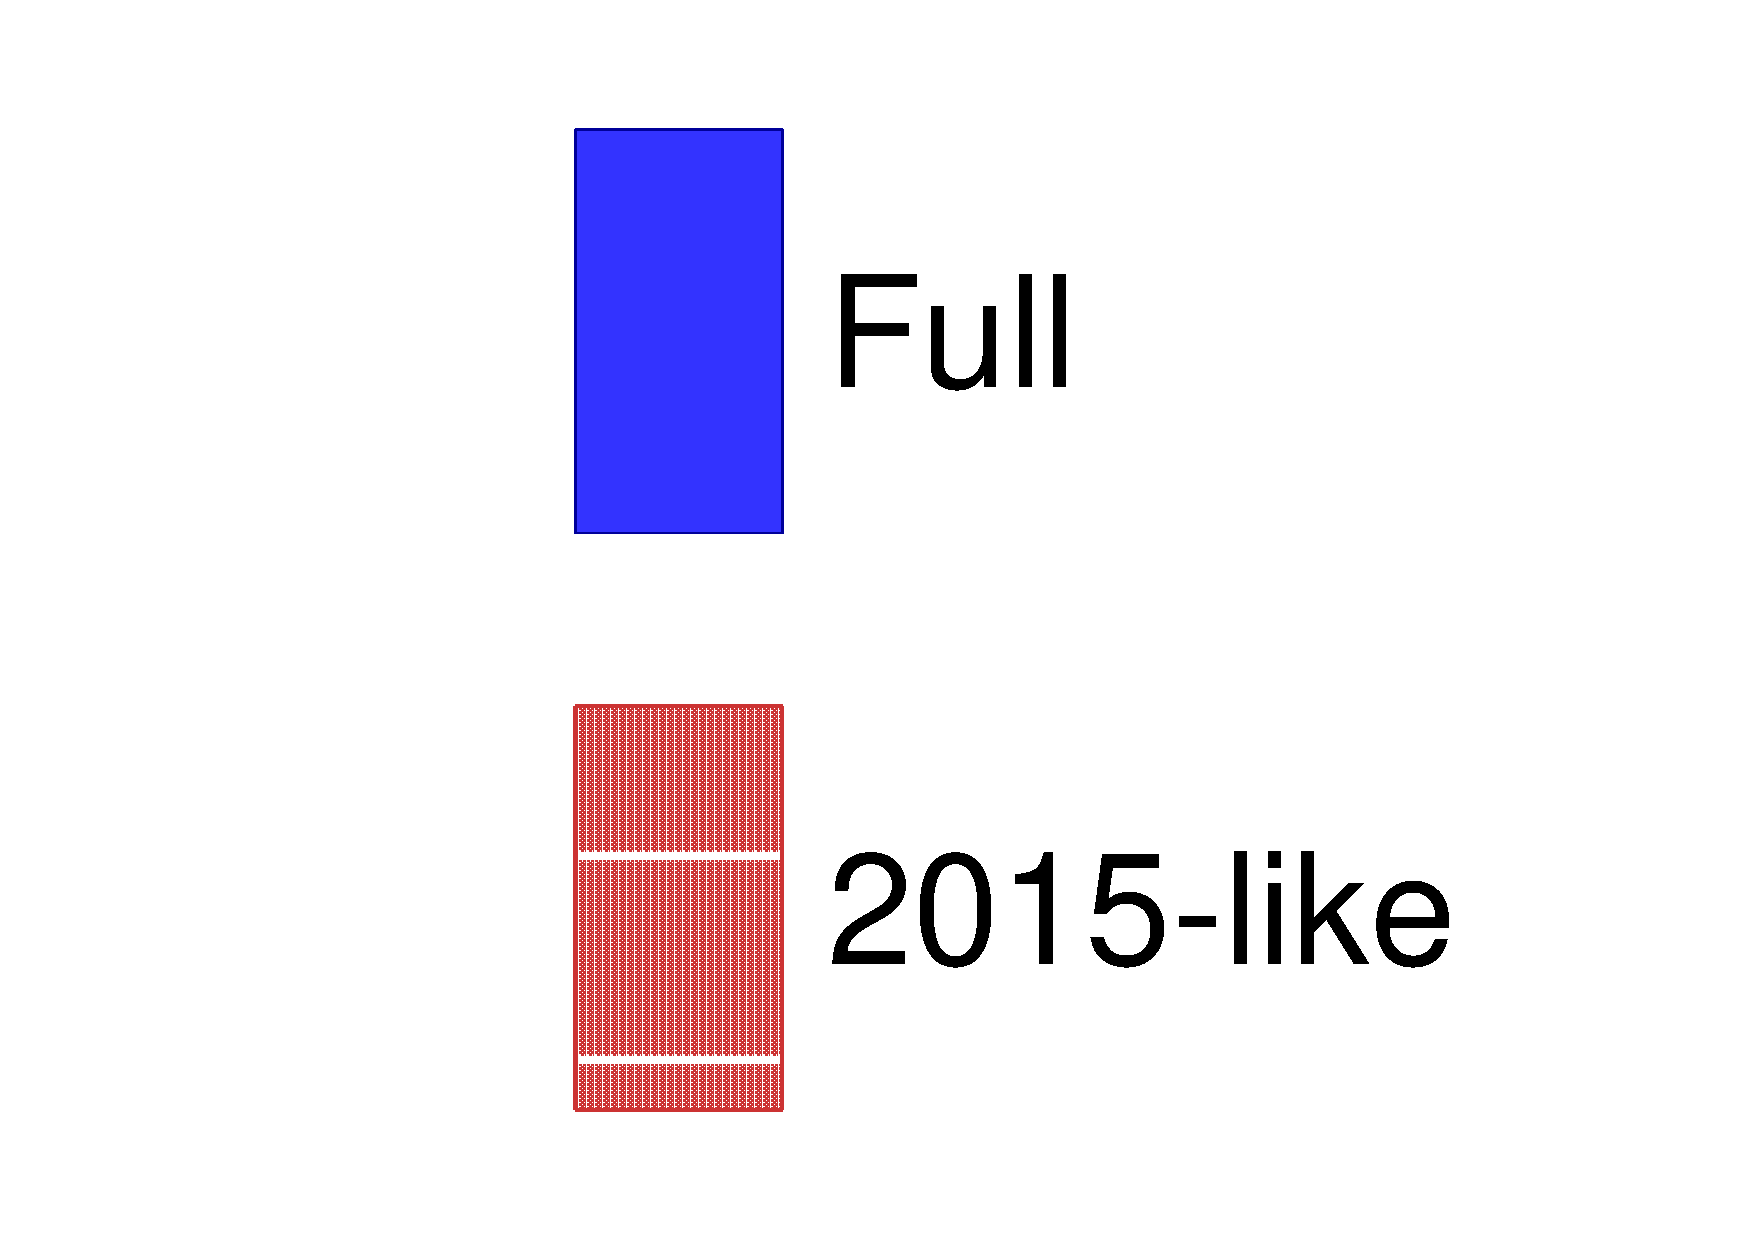
\includegraphics[width=\textwidth, trim={0mm 0mm 0mm 0mm}, clip, page=1]{figures/mach3/data/alt/try_2017_fit_on_sk_spectra_posterior_sk_error_2015like_spectra}
	\end{subfigure}
	\begin{subfigure}[t]{0.32\textwidth}
		\includegraphics[width=\textwidth, trim={0mm 0mm 0mm 0mm}, clip, page=2]{figures/mach3/data/alt/try_2017_fit_on_sk_spectra_posterior_sk_error_2015like_spectra}
	\end{subfigure}
	\begin{subfigure}[t]{0.32\textwidth}
		\includegraphics[width=\textwidth, trim={0mm 0mm 0mm 0mm}, clip, page=3]{figures/mach3/data/alt/try_2017_fit_on_sk_spectra_posterior_sk_error_2015like_spectra}
	\end{subfigure}
		
	\begin{subfigure}[t]{0.32\textwidth}
		\includegraphics[width=\textwidth, trim={0mm 0mm 0mm 0mm}, clip, page=4]{figures/mach3/data/alt/try_2017_fit_on_sk_spectra_posterior_sk_error_2015like_spectra}
	\end{subfigure}
	\begin{subfigure}[t]{0.32\textwidth}
		\includegraphics[width=\textwidth, trim={0mm 0mm 0mm 0mm}, clip, page=5]{figures/mach3/data/alt/try_2017_fit_on_sk_spectra_posterior_sk_error_2015like_spectra}
	\end{subfigure}

\caption{Impact of 2015-like fit on SK spectra compared to full fit}
\label{fig:sk_2015like}
\end{figure}

\subsubsection{FGD1 vs FGD2}
The FGD1 vs FGD2 fit saw numerous difference in parameters: the high energy flux parameters, $M_A^{QE}$, BeRPA, 2p2h shape and pion absorption parameters all moved within 1$\sigma$ of each other, sometimes on the border.

\autoref{fig:sk_fgd1vsfgd2} shows the predicted oscillated SK event distributions for the three fits, in which all the bins agree well inside each other's 1$\sigma$. The largest deviations are again for the $1\text{R}\mu$ FHC and RHC samples with $0.2 < E_{rec}<0.5\text{ GeV}$, in which the full fit sits higher than the individual fits. The $1\text{R}e$ selection do not show much change.
\begin{figure}[h]
	\begin{subfigure}[t]{0.32\textwidth}
		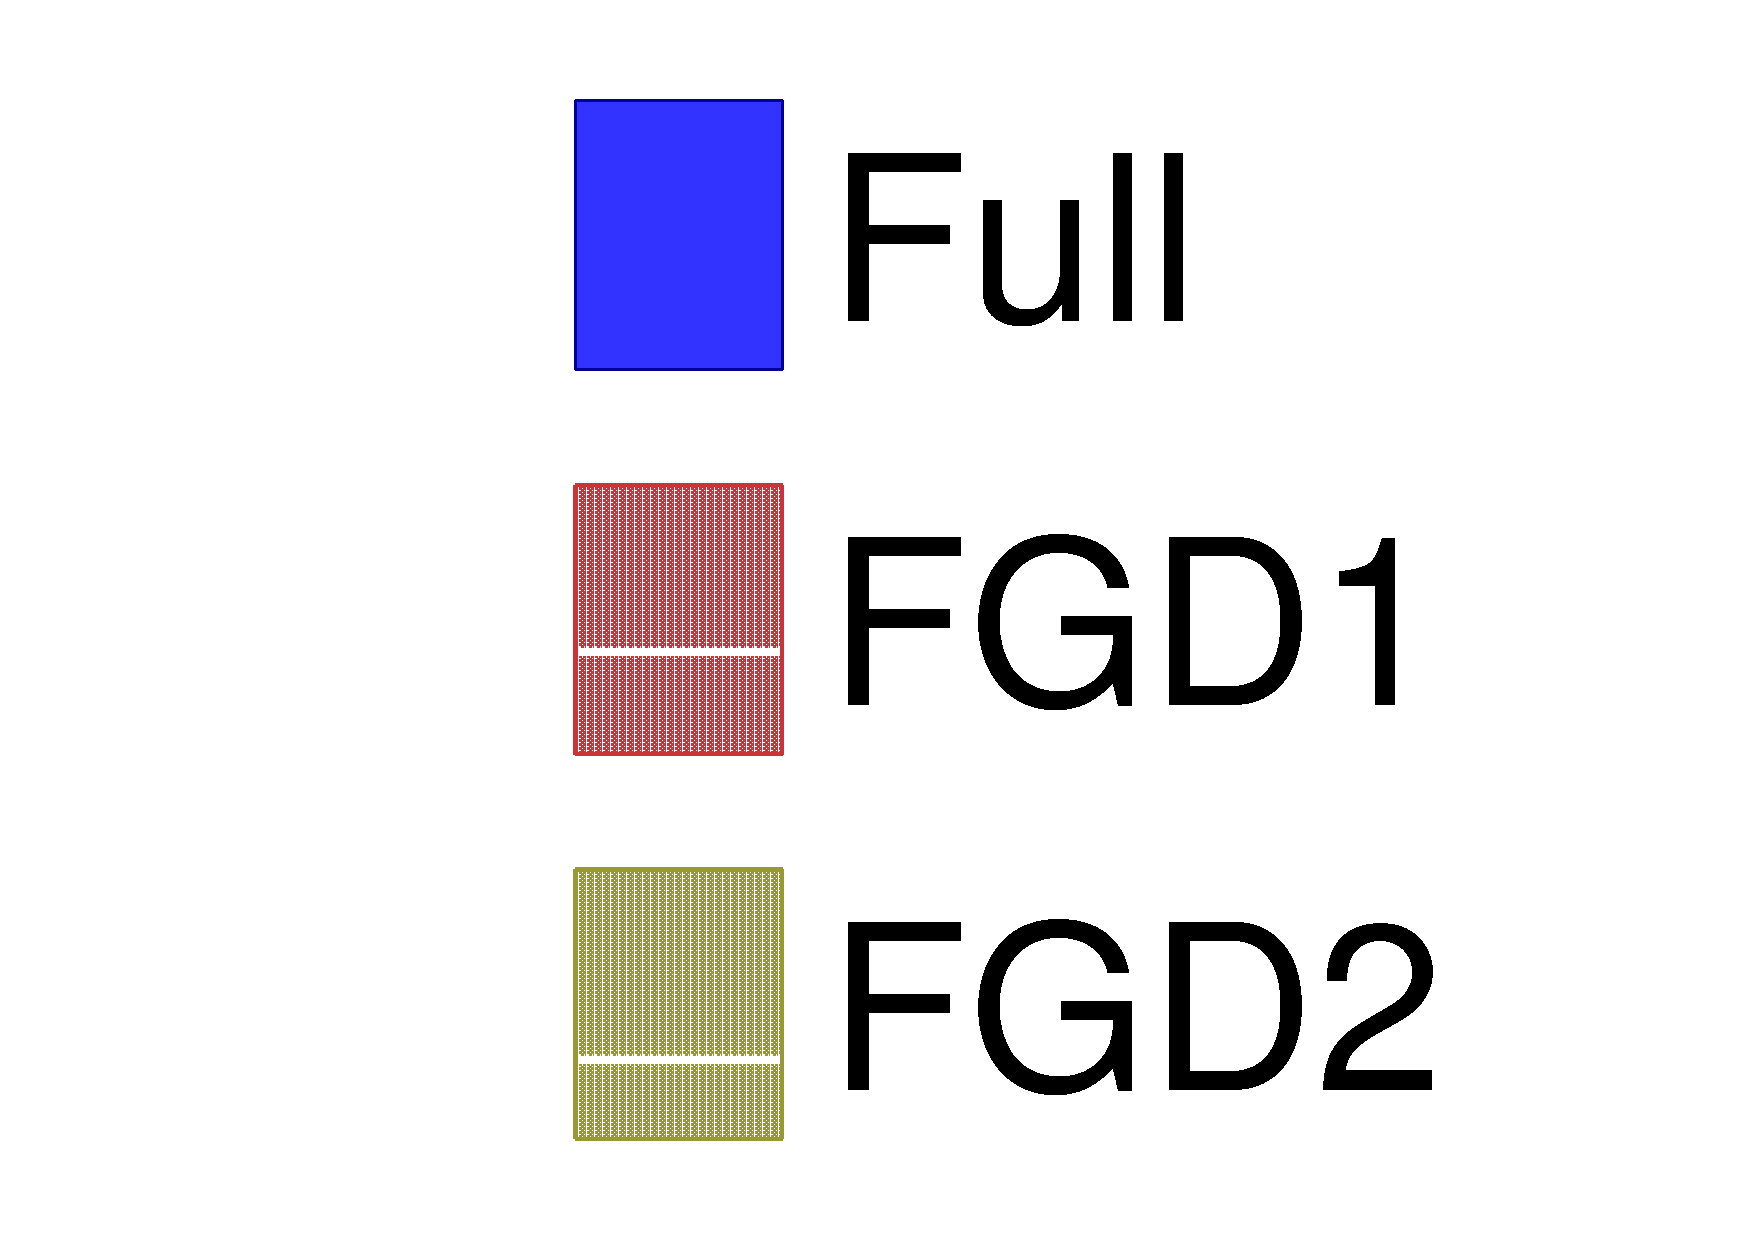
\includegraphics[width=\textwidth, trim={0mm 0mm 0mm 0mm}, clip, page=1]{figures/mach3/data/alt/try_2017_fit_on_sk_spectra_posterior_sk_error_fgd1only_spectra_posterior_sk_error_fgd2only_spectra}
	\end{subfigure}
	\begin{subfigure}[t]{0.32\textwidth}
		\includegraphics[width=\textwidth, trim={0mm 0mm 0mm 0mm}, clip, page=2]{figures/mach3/data/alt/try_2017_fit_on_sk_spectra_posterior_sk_error_fgd1only_spectra_posterior_sk_error_fgd2only_spectra}
	\end{subfigure}
	\begin{subfigure}[t]{0.32\textwidth}
		\includegraphics[width=\textwidth, trim={0mm 0mm 0mm 0mm}, clip, page=3]{figures/mach3/data/alt/try_2017_fit_on_sk_spectra_posterior_sk_error_fgd1only_spectra_posterior_sk_error_fgd2only_spectra}
	\end{subfigure}
	
	\begin{subfigure}[t]{0.32\textwidth}
		\includegraphics[width=\textwidth, trim={0mm 0mm 0mm 0mm}, clip, page=4]{figures/mach3/data/alt/try_2017_fit_on_sk_spectra_posterior_sk_error_fgd1only_spectra_posterior_sk_error_fgd2only_spectra}
	\end{subfigure}
	\begin{subfigure}[t]{0.32\textwidth}
		\includegraphics[width=\textwidth, trim={0mm 0mm 0mm 0mm}, clip, page=5]{figures/mach3/data/alt/try_2017_fit_on_sk_spectra_posterior_sk_error_fgd1only_spectra_posterior_sk_error_fgd2only_spectra}
	\end{subfigure}
	\caption{Impact of FGD1 vs FGD2 fit on SK spectra compared to full fit}
	\label{fig:sk_fgd1vsfgd2}
\end{figure}

\subsubsection{FHC vs RHC}
The FHC (run 2 to 4) vs RHC (run 5 to 6) fits generally showed the RHC samples agreeing better with the priors through the parameter space. For the interaction parameters we saw significantly different values of $M_A^{QE}$, 2p2h shape, BeRPA, $M_A^{RES}$, non-resonant $I_{1/2}$ and some pion FSI parameters, and the uncertainties were much larger on the RHC data due to low statistics. This was worrying because unmodelled neutrino/anti-neutrino differences at Super-Kamiokande can potentially be soaked up in $\delta_{CP}$, exaggerating its constraints.

\autoref{fig:sk_fhcvsrhc} shows the three fits for the SK selections, where the differences are large albeit for FHC within 1$\sigma$ of each other and the full fit. The FHC fit agrees well with the full fit for the FHC selections and the RHC fit agrees slightly worse with the full fit for the RHC selections.

The FHC fit prediction for the RHC samples has very large associated uncertainties and has a much larger normalisation than the full and RHC-only prediction, which would primarily affect the $\theta_{13}$ and $\theta_{23}$ mixing angles. The RHC-only prediction for FHC is consistently higher: for $1\text{R}\mu$ the effect is most noticeable in the above the oscillation dip at $E_{rec}\sim0.6\text{ GeV}$, the $1\text{R}e$ shows most difference in the low $E_{rec}$ range, and again the $1\text{R}e1\text{d}e$ selection instead shows the largest effect at higher $E_{rec}$.

This study highlights the importance of collecting similar numbers of $\nu$ and $\bar{\nu}$ at ND280 and SK.
\begin{figure}[h]
	\begin{subfigure}[t]{0.32\textwidth}
		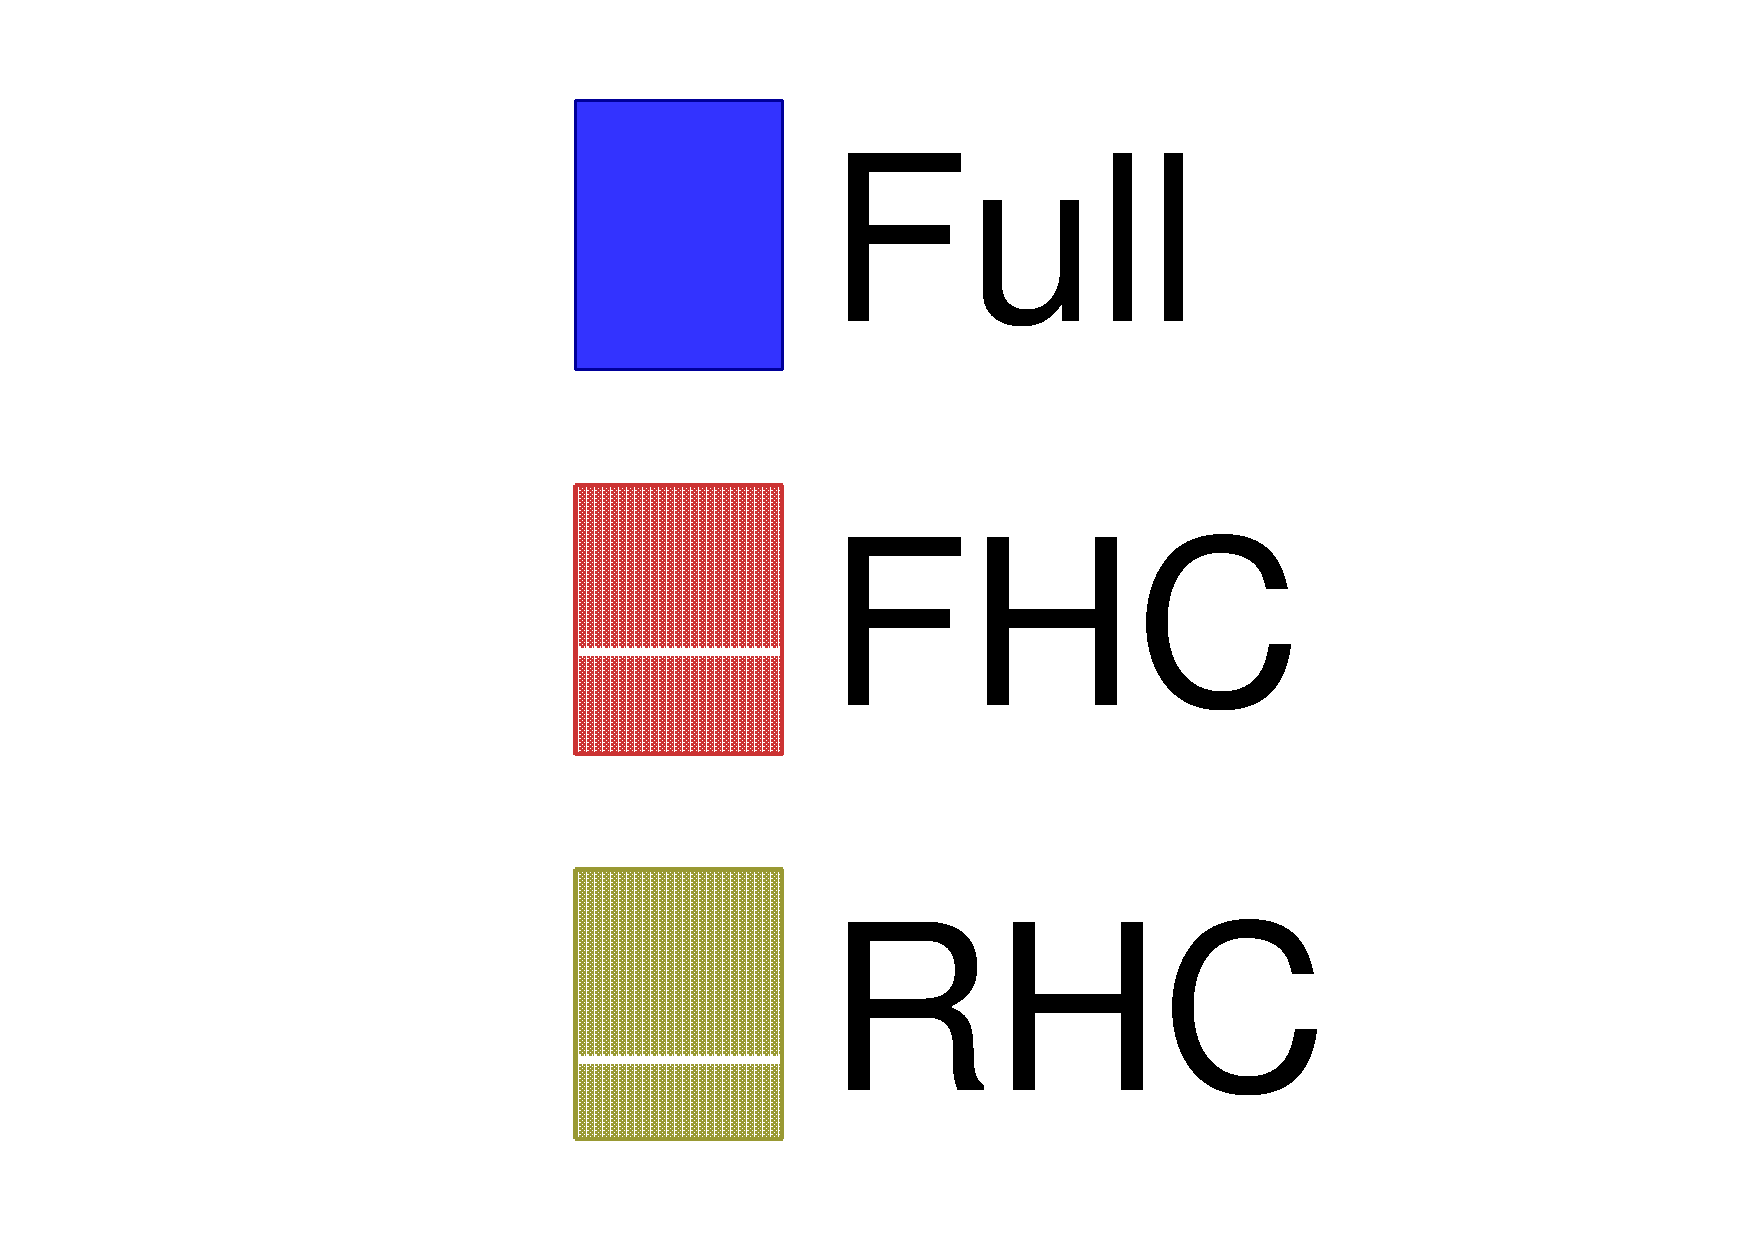
\includegraphics[width=\textwidth, trim={0mm 0mm 0mm 0mm}, clip, page=1]{figures/mach3/data/alt/try_2017_fit_on_sk_spectra_posterior_sk_error_run2to4_spectra_posterior_sk_error_run5to6_spectra}
	\end{subfigure}
	\begin{subfigure}[t]{0.32\textwidth}
		\includegraphics[width=\textwidth, trim={0mm 0mm 0mm 0mm}, clip, page=2]{figures/mach3/data/alt/try_2017_fit_on_sk_spectra_posterior_sk_error_run2to4_spectra_posterior_sk_error_run5to6_spectra}
	\end{subfigure}
	\begin{subfigure}[t]{0.32\textwidth}
		\includegraphics[width=\textwidth, trim={0mm 0mm 0mm 0mm}, clip, page=3]{figures/mach3/data/alt/try_2017_fit_on_sk_spectra_posterior_sk_error_run2to4_spectra_posterior_sk_error_run5to6_spectra}
	\end{subfigure}
	
	\begin{subfigure}[t]{0.32\textwidth}
		\includegraphics[width=\textwidth, trim={0mm 0mm 0mm 0mm}, clip, page=4]{figures/mach3/data/alt/try_2017_fit_on_sk_spectra_posterior_sk_error_run2to4_spectra_posterior_sk_error_run5to6_spectra}
	\end{subfigure}
	\begin{subfigure}[t]{0.32\textwidth}
		\includegraphics[width=\textwidth, trim={0mm 0mm 0mm 0mm}, clip, page=5]{figures/mach3/data/alt/try_2017_fit_on_sk_spectra_posterior_sk_error_run2to4_spectra_posterior_sk_error_run5to6_spectra}
	\end{subfigure}
	
	\caption{Impact of FHC vs RHC fit on SK spectra compared to full fit}
	\label{fig:sk_fhcvsrhc}
\end{figure}

\section{MCMC stability}
In the black box situation, the best diagnostic is to run the chain
for a very long time — like from the time the paper is submitted
until referees reports arrive. Geyer, University of Minnesota

\clearpage